% Created 2021-01-24 Sun 22:49
% Intended LaTeX compiler: pdflatex
\documentclass[11pt]{article}
\usepackage[utf8]{inputenc}
\usepackage[T1]{fontenc}
\usepackage{graphicx}
\usepackage{grffile}
\usepackage{longtable}
\usepackage{wrapfig}
\usepackage{rotating}
\usepackage[normalem]{ulem}
\usepackage{amsmath}
\usepackage{textcomp}
\usepackage{amssymb}
\usepackage{capt-of}
\usepackage{hyperref}
\usepackage{minted}
\hypersetup{colorlinks=true, linkcolor=black, filecolor=red, urlcolor=blue}
\usepackage[turkish]{babel}
\author{Eren Hatırnaz}
\date{31 Aralık 2019}
\title{Yazılım Gündemi - 23\\\medskip
\large 23-29 Aralık 2019}
\hypersetup{
 pdfauthor={Eren Hatırnaz},
 pdftitle={Yazılım Gündemi - 23},
 pdfkeywords={},
 pdfsubject={},
 pdfcreator={Emacs 27.1 (Org mode 9.3)},
 pdflang={Turkish}}
\begin{document}

\maketitle
\tableofcontents \clearpage\shorthandoff{=}

\begin{center}
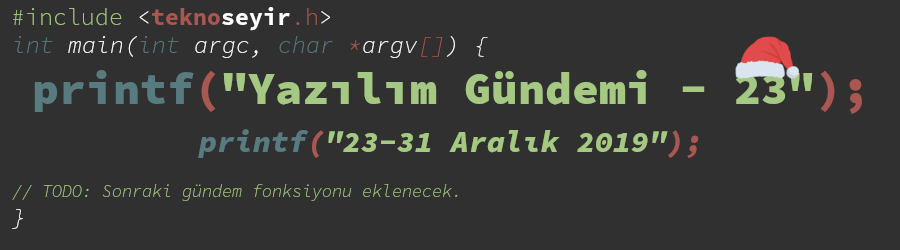
\includegraphics[width=.9\linewidth]{gorseller/yazilim-gundemi-banner.png}
\end{center}

\begin{center}
\href{../22/yazilim-gundemi-22.pdf}{< Önceki Gündem} | \textbf{23-29 Aralık 2019} | \href{../../2020/01/yazilim-gundemi-2020-01.pdf}{Sonraki Gündem >}

\href{https://teknoseyir.com/blog/yazilim-gundemi-23-23-31-aralik-2019}{TeknoSeyir'de Oku}
\end{center}

\section{2020 dönemi için Python yönetim konseyi \href{https://www.python.org/dev/peps/pep-8101/}{üyeleri seçildi}}
\label{sec:org4d4487c}
\begin{center}

\includegraphics[height=2cm]{gorseller/python-yonetim-konseyi.png}
\end{center}

Python uzun zamandır geliştirilen bir programlama dili olduğu için haliyle
yönetimi için de bazı kararlar alınması gerekiyordu. Kısaca tarihçesinden
bahsetmek gerekirse: Guido van Rossum (Python dilinin yaratıcısı), 2018'in
temmuz ayında Python mail grubuna bazı kararları verirken yorulduğunu ve artık
karar verici konumunda olmak istemediğini belirten \href{https://mail.python.org/pipermail/python-committers/2018-July/005664.html}{bir mail yazıyor} ve
topluluğa "kendi yönetim şeklinizi kendiniz belirleyin" diyor. Bunun üzerine
python ana geliştirici takımı da çeşitli yönetim modelleri \href{https://www.python.org/dev/peps/pep-8000/}{üzerine tartışmalar
yaptılar} ve "\href{https://www.python.org/dev/peps/pep-8016/}{PEP 8016 - The Steering Council Model}" sistemi üzerinde karar
kıldılar. Daha sonra bu model üzerinde biraz değişiklikler yaparak bugün
geçerli olan haline getirdiler: \href{https://www.python.org/dev/peps/pep-0013/}{PEP 13 - Python Language Governance}. Guio van
Rossum yine yönetim kurulunun bir üyesi olarak seçilmişti.

Yönetim konseyi modelinden de kısaca bahsedeyim havada kalmasın. Bu modele göre
yönetim konseyi 5 kişiden oluşabilir. Seçilen bu 5 kişi ise Python dilinin
kalitesini ve stabilitesini sürdürmekte yükümlü olmasının yanı sıra, Python ana
geliştirici takımı ve Python Software Foundation arasındaki ilişkiyi kurma,
gerektiğinde kod yazarak katkı sağlama, uygun karar verme süreçlerini kurmak
gibi görevlerle birlikte PEP'leri kabul etmek ya da reddetmek, davranış
kurallarını güncelleyebilmek gibi güçleri de mevcut. Bu yönetim şekliyle ilgili
diğer detaylar için \href{https://www.python.org/dev/peps/pep-0013/\#history}{PEP 13 sayfası}nı ziyaret edebilirsiniz.

Kasım ayında gerçekleşen aday belirleme süreçlerinden sonra bu ayın başlarında
oylama işlemi gerçekleştirildi ve yeni yönetim konseyi üyeleri belli oldu:
\begin{itemize}
\item Barry Warsaw (50 oy),
\item Brett Cannon (54 oy),
\item Carol Willing (54 oy),
\item Thomas Wouters (40 oy),
\item Victor Stinner (38 oy).
\end{itemize}

Adayları sadece Python ana geliştirici takımı üyeleri önerebiliyor, eğer kişi
Python ana geliştirici takımı üyesi ise kendini de önerebiliyor. Bu bağlamda
Guido van Rossum da yönetim kurulu üyesi için önerilmişti fakat \href{https://discuss.python.org/t/steering-council-nomination-guido-van-rossum-2020-term/2657/11}{yazdığı forum
mesajı ile adaylıktan çekildi} ama "yine de ben buralardayım katkı sunmaya, soru
yanıtlamaya devam edeceğim" dedi.

Yeni yönetim kurulu üyelerine başarılar dilerim. :)

Yeni yıla girerken daha önceki yazılım gündeminde de duyurduğum gibi Python
2'nin 1 Ocak 2020'den itibaren desteklenmeyeceği tekrar hatırlatmış olayım.
Python 2'nin \href{https://pythonclock.org/}{ölümü için geri sayım} da burada gerçekleşiyor. Elveda Python
2.7\ldots{}
\section{Ruby 2.7 \href{https://www.ruby-lang.org/en/news/2019/12/25/ruby-2-7-0-released/}{sürümü yayınlandı}}
\label{sec:orgc6eb2cb}
Akıcı syntax'ından dolayı çok beğendiğim fakat uzun zamandır yazmaya fırsatım
olmayan Ruby programlama dilinin 2.7.0 sürümü bu hafta yayınlandı. Zaten
geçtiğimiz haftaki gündem yazısında da belirtmiştim bu hafta yayınlanacağını.
Ruby 3 ile değişecek olan argüman işleme sisteminden ve Ruby 2.7'deki
etkilerinden zaten geçen hafta \href{../22/yazilim-gundemi-22.pdf}{Yazılım Gündemi - 22} yazısında bahsetmiştim.
Onun dışındaki yeniliklere bakalım:

\subsection{Pattern Matching [Deneysel]}
\label{sec:orga2fa8cd}
Henüz deneysel olarak eklenmiş bu özellik ile birlikte artık objelerin
içerisindeki istediğiniz yapılara göre eşleme yapabileceksiniz. Örnek verirsem
daha iyi anlaşılacak. Şöyle ki, elinizde bir JSON verisi var diyelim:
\newpage
\begin{minted}[breaklines=true,breakanywhere=true,frame=lines, linenos, label=JSON, labelposition=topline]{json}
{
  "isim": "Ahmet",
  "yas": "45",
  "cocuklar": [{
    "isim": "Mehmet",
    "yas": 5
  }]
}
\end{minted}
ve kendi ismi Ahmet, çocuğunun ismi Mehmet olan birinin verisini çekip çocuğun
yaşını yazdırmak istiyorsunuz. Eskiden bu şekilde yapıyorduk:
\begin{minted}[breaklines=true,breakanywhere=true,frame=lines, linenos, label=Ruby, labelposition=topline]{ruby}
kisi=JSON.parse(json, symbolize_names: true)
if kisi[:isim] == "Ahmet"
  cocuklar = kisi[:cocuklar]
  if cocuklar.length == 1 && cocuklar[0][:name] == "Mehmet"
    puts cocuklar[0][:yas] # => 5
  end
end
\end{minted}
Daha karmaşık JSON verilerinde bu kod parçasının alacağı hali varın siz
düşünün\ldots{} ya da yok düşünmenize gerek yok Ruby 2.7 var:
\begin{minted}[breaklines=true,breakanywhere=true,frame=lines, linenos, label=Ruby, labelposition=topline]{ruby}
case JSON.parse(json, symbolize_names: true)
in {isim: "Ahmet", cocuklar: [{isim: "Mehmet", yas: cocuk_yas}]}
    puts cocuk_yas # => 5
end
\end{minted}
Bu kadar kolay!

Bu özellik hakkında daha fazla bilgi için \href{https://speakerdeck.com/k\_tsj/pattern-matching-new-feature-in-ruby-2-dot-7}{bu adresdeki sunum dosyası}nı
inceleyebilirsiniz.
\subsection{REPL iyileştirmeleri}
\label{sec:org3183d9e}
REPL sistemi birçok popüler scripting dilinde artık olmazsa olmazlardan biri
haline geldi. Açılımı Read-Eval-Print-Loop olan bu özellik sayesinde
terminalinizinden ilgili programlama dilini interaktif bir şekilde
kullanabiliyorsunuz. Ruby dilinde de bu internaktif deneyim için \texttt{irb} aracını
kullanıyorduk. Ruby 2.7 ile bu araca yeni özellikler gelmiş.

\url{gorseller/ruby-27-irb.gif}

irb aracına çok satırlı düzenleme özelliği gelmiş. Bununla birlikte kod
renklendirme de eklenmiş. \texttt{rdoc} entegrasyonu da sağlanmış.
\section{\href{https://2019.stateofjs.com/}{JavaScript'in Durumu 2019} anketi sonuçları yayınlandı}
\label{sec:orgaa2f0a8}
JavaScript her geçen gün popülerliği daha da artan ve kullanılan bir dil. Her
ne kadar bazı alanlara zorla sokulması hoşuma gitmese de şu an için -en azından
sektör içerisindeki kullanıma göre- alternatifi yok gibi bir şey
(WebAssembly'den yana umudum var). Her yıl düzenlenen JavaScript'in Durumu
(State of JavaScript) anketi bu sene de düzenlendi ve sonuçları çok güzel
grafiklerle birlikte duyuruldu. Bu aslında geçen haftanın haberiydi fakat yazı
daha fazla uzamasın diye bu haftaya ertelemiştim. Öyleyse birkaç grafiği
birlikte inceleyelim.

\subsection{JavaScript'e dönüştürülebilen diller}
\label{sec:orgc8ff263}
\begin{center}
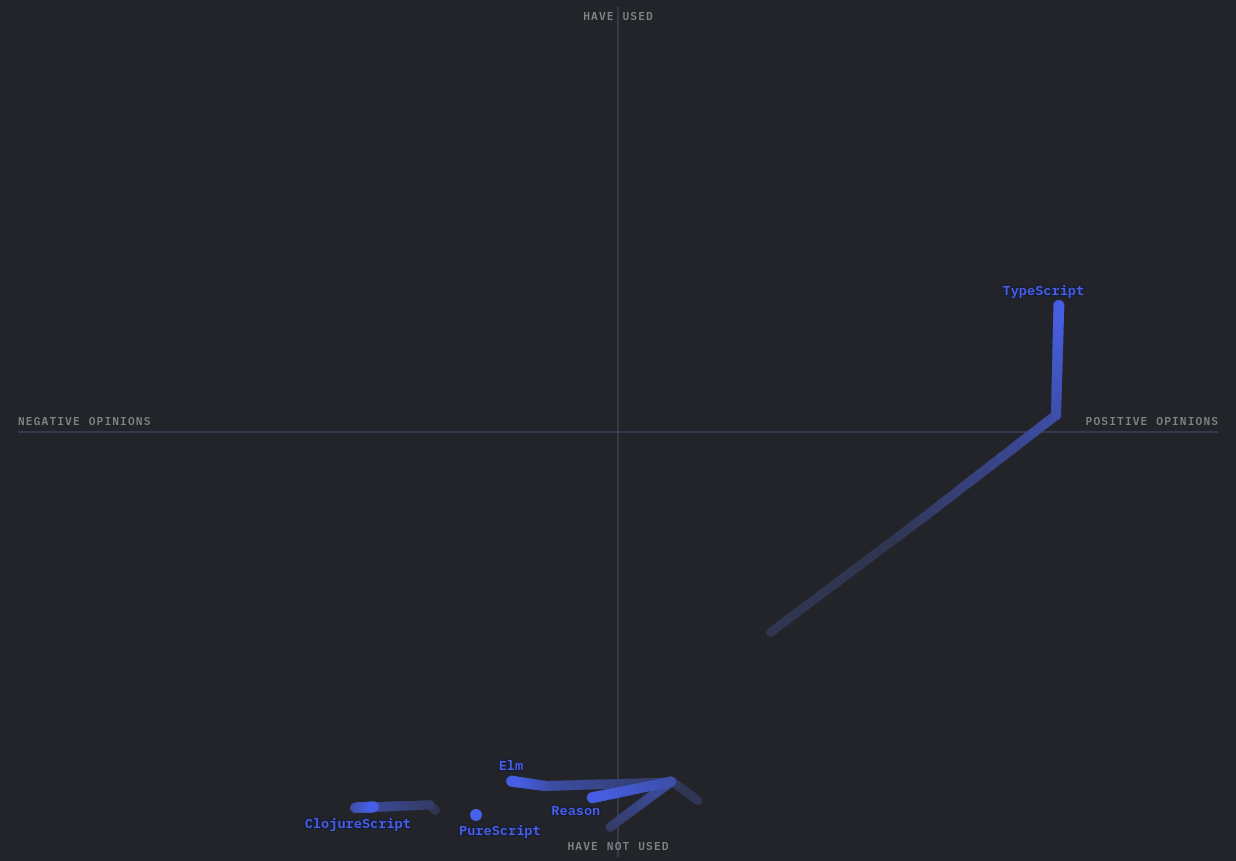
\includegraphics[width=.9\linewidth]{gorseller/sojs-javascript-flavors.png}
\end{center}

Bu grafikteki her noktanın arkasındaki akış 2016 yılından bugüne aldığı yolu
gösteriyor. Buna göre bakacak olursak: \href{https://www.typescriptlang.org/}{TypeScript}'in liderliği çok açık
ortada zaten diğer dillerin kullanımı da çok düşük. Ben bir zamanlar
\href{https://coffeescript.org/}{CoffeeScript} dilini bir süre kullandım, hatta bu dille yazılmış bir açık
kaynak Chrome eklentisine bayağı bir katkı sağladım fakat artık grafikte yeri
bile yok. Açıkcası yazmaktan hoşlandığım bir dildi fakat şu an olsa yazar
mıyım bilemiyorum.
\subsection{Front-End kütüphaneleri}
\label{sec:orge2aa9e5}
\begin{center}
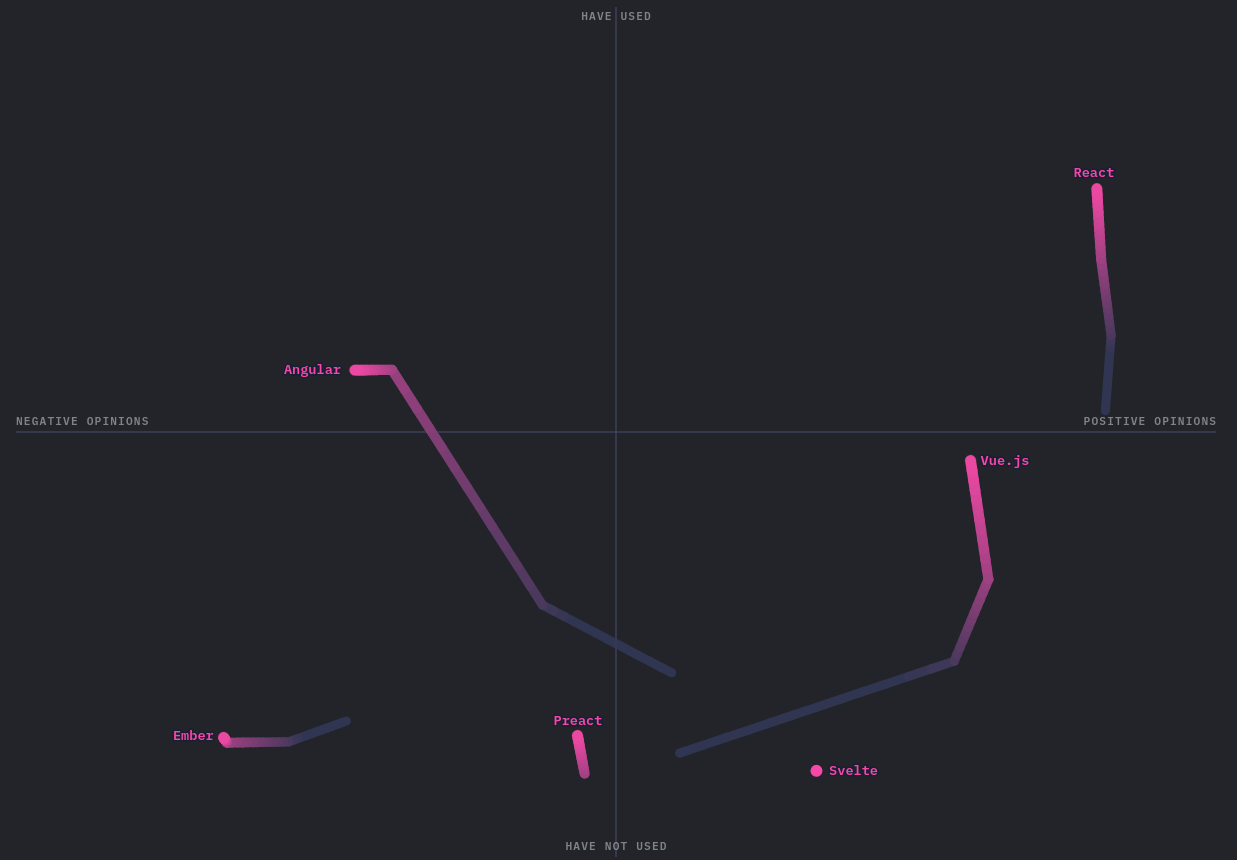
\includegraphics[width=.9\linewidth]{gorseller/sojs-front-end.png}
\end{center}

Açıkcası \href{https://reactjs.org/}{React}'in yükselişi için pek sürpriz oldu diyemem ama bu sene ortaya
çıkan \href{https://svelte.dev/}{Svelte}'ye bu kadar pozitif bakılması beni şaşırttı. Bunların dışında
\href{https://angular.io/}{Angular}'ın kullanımı zaman içinde artmış fakat negatif tarafa düşmüş. Bir ara
denemiştim ben de fakat fazla karışık gelmişti. Diğer kütüphanelerle ilgili
pek bir bilgim yok.

İnsanların en çok memnun oldukları front-end kütüphaneleri sıralaması ise bu
şekilde:

\begin{center}
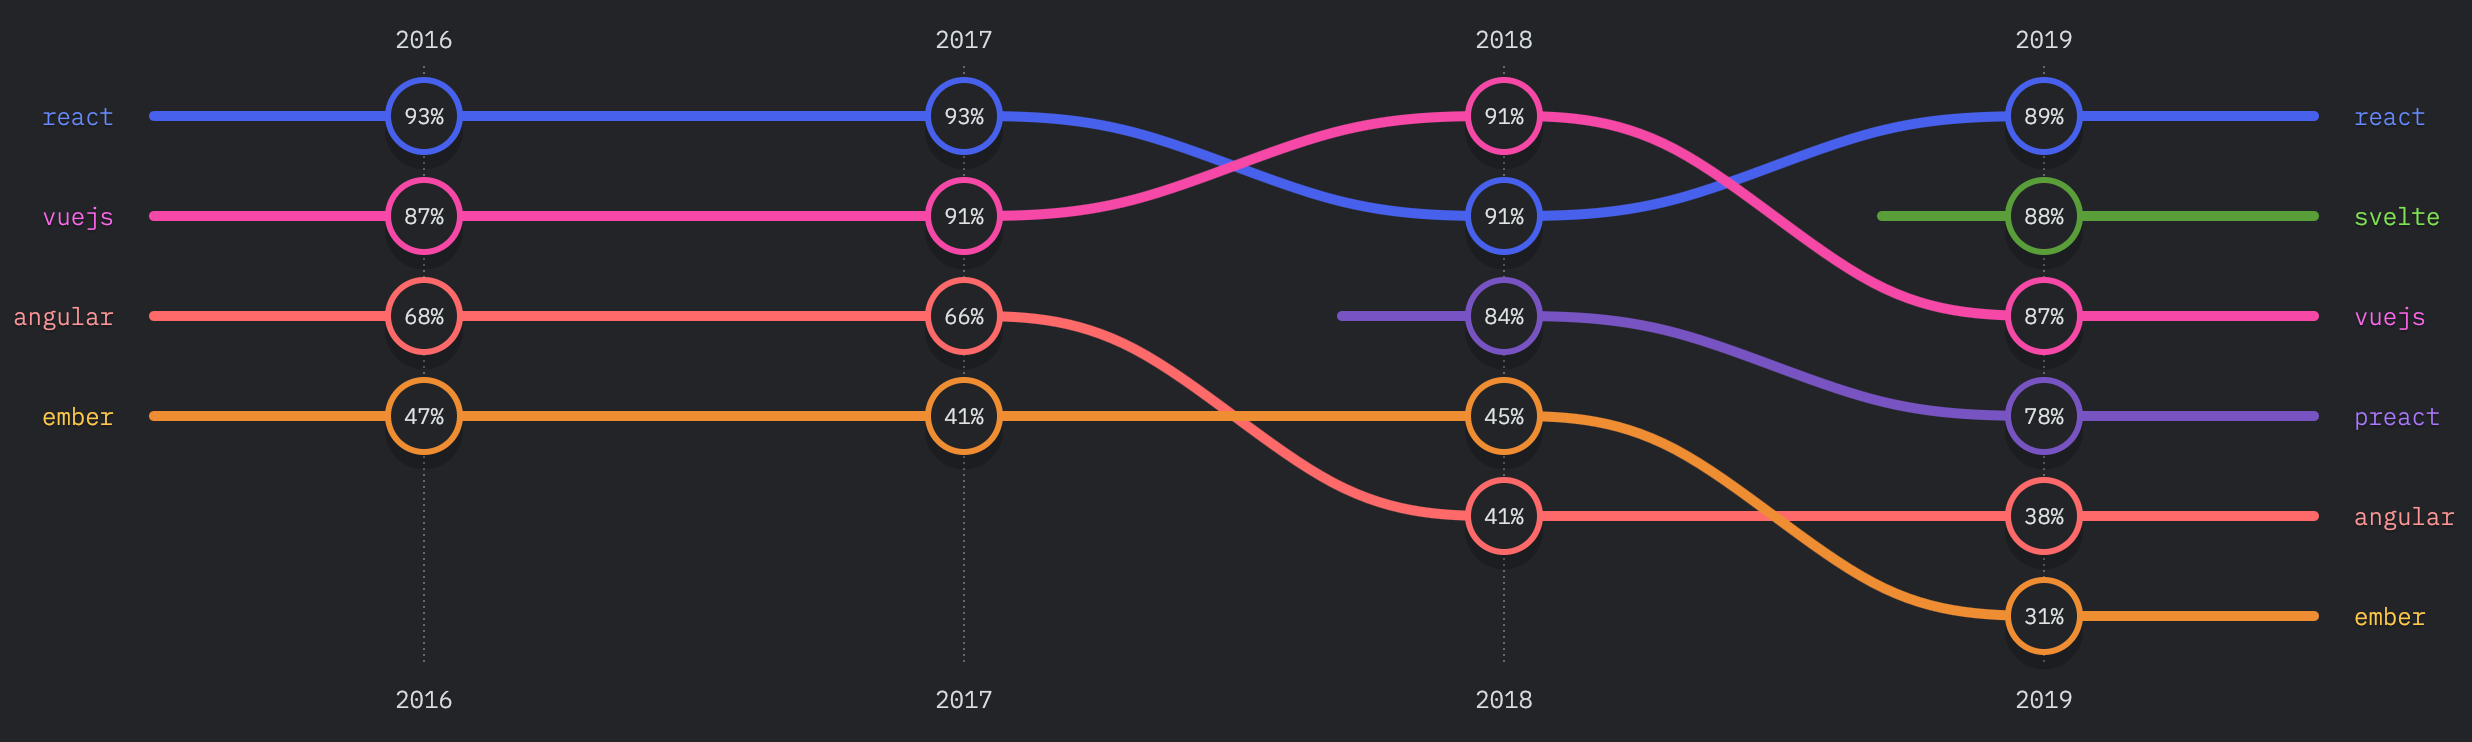
\includegraphics[width=.9\linewidth]{gorseller/sojs-front-end-memnuniyet.png}
\end{center}

Diğer kategorilerdeki istatistikleri de paylaşmak isterdim fakat yazısı çok
uzatmış olurum. O yüzden daha fazla istatistik ve bilgi için konu başlığına
eklediğim bağlantıya tıklayabilirsiniz.

Alternatif olarak da \href{https://levelup.gitconnected.com/a-recap-of-frontend-development-in-2019-1e7d07966d6c}{şu blog yazısı}ndaki istatistiklere göz atabilirsiniz.
\section{Java 14 Feature-freeze \href{https://www.infoq.com/news/2019/12/java14-feature-freeze/}{sürecine girdi}}
\label{sec:org9508cf1}
Java programlama dilinin 14 numaralı sürümü için feature-freeze sürecine
girildi. Yani artık programlama diline yeni özellik eklenmeyecek ve sürümün
yayınlanması için çalışmalar yapılacak. JDK 14 "Rampdown Phase One" ismini
verdikleri \href{https://openjdk.java.net/projects/jdk/14/}{sürece girmiş}. Release Candidate 1 sürümünün 6 şubat 2020, Release
Candidate Final sürümünün ise 20 Şubat 2020 tarihinde yayınlanması
planlanırken, genel erişilebilirlik için de 17 mart 2020 tarihi verilmiş. Kabul
edilen JEP'ler (Java Enhancement Proposals) ise bu şekilde:

\begin{itemize}
\item JEP 345: \href{https://openjdk.java.net/jeps/345}{NUMA-Aware Memory Allocation for G1}
\item JEP 349: \href{https://openjdk.java.net/jeps/349}{JFR Event Streaming}
\item JEP 352: \href{https://openjdk.java.net/jeps/352}{Non-Volatile Mapped Byte Buffers}
\item JEP 358: \href{https://openjdk.java.net/jeps/358}{Helpful NullPointerExceptions}
\item JEP 361: \href{https://openjdk.java.net/jeps/361}{Switch Expressions (Standard)}
\item JEP 364: \href{https://openjdk.java.net/jeps/364}{ZGC on macOS}
\item JEP 365: \href{https://openjdk.java.net/jeps/365}{ZGC on Windows}
\end{itemize}

JDK 14'de Preview olarak eklenecek özellikler ise bu şekilde:
\begin{itemize}
\item JEP 305: \href{https://openjdk.java.net/jeps/305}{Pattern Matching for instanceof (Preview)}
\item JEP 343: \href{https://openjdk.java.net/jeps/343}{Packaging Tool (Incubator)}
\item JEP 368: \href{https://openjdk.java.net/jeps/368}{Text Blocks (Second Preview)}
\item JEP 370: \href{https://openjdk.java.net/jeps/370}{Foreign-Memory Access API (Incubator)}
\item JEP 359: \href{https://openjdk.java.net/jeps/359}{Records (Preview)}
\end{itemize}

Dilden kaldırılan ya da deprecate olan özellikler:
\begin{itemize}
\item JEP 362: \href{https://openjdk.java.net/jeps/362}{Deprecate the Solaris and SPARC Ports}
\item JEP 366: \href{https://openjdk.java.net/jeps/366}{Deprecate the ParallelScavenge + SerialOld GC Combination}
\item JEP 363: \href{https://openjdk.java.net/jeps/363}{Remove the Concurrent Mark Sweep (CMS) Garbage Collector}
\item JEP 367: \href{https://openjdk.java.net/jeps/367}{Remove the Pack200 Tools and API}
\end{itemize}

Detaylıca incelemelerini önümüzdeki yazılım gündemi yazılarına bırakıyorum.
\section{Yaklaşan Etkinlikler}
\label{sec:org9ef6bad}
\begin{longtable}{|p{8cm}|l|l|}
\hline
Etkinlik İsmi & Yeri & Tarihi\\
\hline
\endfirsthead
\multicolumn{3}{l}{Önceki sayfadan devam ediyor} \\
\hline

Etkinlik İsmi & Yeri & Tarihi \\

\hline
\endhead
\hline\multicolumn{3}{r}{Devamı sonraki sayfada} \\
\endfoot
\endlastfoot
\hline
\href{https://www.meetup.com/Hukuk-ve-Teknoliji-Meetup-Grubu/events/267223619/}{KVKK ve GDPR Kapsamında Veri Güvenliği} & Ankara & 3 Ocak 18:30\\
\href{https://www.meetup.com/Yaz\%25C4\%25B1l\%25C4\%25B1m-Geli\%25C5\%259Ftiricileri-Geli\%25C5\%259Ftirme/events/266380738/}{Asp.net MVC Framework Workshop} & İstanbul & 3 Ocak 19:00\\
\href{https://www.meetup.com/Coffee-And-React-Native-\%25C4\%25B0stanbul/events/vzxzkrybccbgb/}{Coffee and React Native} & İstanbul & 4 Ocak 11:00\\
\href{https://www.meetup.com/CodeHAP-Habbit-Art-Passion/events/267414497/}{Reactive Programming} & İstanbul & 8 Ocak 19:20\\
\href{https://www.meetup.com/Gorsellestirme-Teknolojileri/events/266312464/}{Sanal Gerçeklik ve Render ile Görselleştirme Teknolojileri} & İstanbul & 9 Ocak 19:00\\
\hline
\end{longtable}

\textbf{\href{https://kamp.linux.org.tr/2020/kis/}{Mustafa Akgül Özgür Yazılım Kış Kampı} katılımcı başvuruları 1 ocak tarihinde
başlayacak.}
\section{Diğer Haberler}
\label{sec:org15fe850}
\begin{itemize}
\item \href{https://blog.scottlogic.com/2019/12/24/webassembly-2019.html}{WebAssembly için 2019 yılı özeti} yayınlandı.
\item JetBrains, MPS 2019.3 \href{https://blog.jetbrains.com/mps/2019/12/mps-2019-3-is-released/}{sürümünü duyurudu}.
\item PyPy 7.3.0 \href{https://morepypy.blogspot.com/2019/12/pypy-730-released.html}{sürümü yayınlandı}.
\item Common Lisp derleyicisi SBCL, 2.0.0 \href{http://www.sbcl.org/all-news.html?2.0.0\#2.0.0}{sürümünü yayınladı}.
\item IntelliJ tabanlı IDE olan IntelliJ Rust, yeni bir \href{https://intellij-rust.github.io/2019/12/30/changelog-113.html}{changelog yayınladı}.
\item Rust ile yazılmış 2D grafik kütüphanesi lyon, 0.15.0 \href{https://nical.github.io/posts/new-tessellator.html}{sürümünü duyurdu}.
\item Rust için SQL kütüphanesi SQLx 0.1.1 \href{https://github.com/launchbadge/sqlx?utm\_name=iossmf}{sürümüyle ortaya çıktı}.
\item Go ile yazılmış JSON sorgu aracı JQL \href{https://github.com/cube2222/jql}{yayınlandı}.
\item API test aracı vREST NG, 1.1.0 \href{https://ng.vrest.io/change-log}{sürümünü duyurdu}.
\item Platformlar-arası uygulama geliştirmeye yarayan framework NeutralinoJS,
1.3.0 \href{https://github.com/neutralinojs/neutralinojs/releases/tag/v1.3.0?utm\_name=iossmf}{sürümünü yayınladı}.
\item C++ terminal uygulamalarında metin tabanlı tablolar oluşturmaya yarayan
kütüphane yayınlandı: \href{https://github.com/p-ranav/tabulate}{Tabulate}.
\item Scheme dili için geliştirilmiş web framework sistemi \href{https://web-artanis.com/}{GNU Artanis}, 0.4.1
\href{https://lists.gnu.org/archive/html/artanis/2019-12/msg00000.html}{sürümünü yayınladı}. \href{https://nalaginrut.com/archives/2019/12/25/what\%2527s\%2520new\%2520in\%2520gnu\%2520artanis\%25200.4.1}{Yeniliklerle ilgili blog yazısı}
\item Rust için HTTP istemcisi reqwest, v0.10 \href{https://seanmonstar.com/post/189960517042/reqwest-v010}{sürümünü duyurdu}.
\item KDE Fremawork 6 için \href{https://ervin.ipsquad.net/blog/2019/12/28/kf6-progress-report-december-solstice-edition/}{durum raporu yayınlandı}.
\item Bottender 1.1.0 \href{https://bottender.js.org/blog/2019/12/27/bottender-1\_1}{sürümü çıktı}.
\end{itemize}
\section{Credits}
\label{sec:org3d84452}
\begin{itemize}
\item Banner görselinde kullandığım \href{https://www.flaticon.com/free-icon/hat\_744546}{noel baba şapkası} \href{https://www.flaticon.com/}{FlatIcons} sitesinden,
\href{https://www.flaticon.com/authors/vectors-market}{Vectors Market} tarafından tasarlanmıştır.
\item Python yönetim konseyi haberinin başlık görselindeki \href{https://www.flaticon.com/free-icon/elections\_1582013}{oy sandığı ikonu}
\href{https://flaticon.com}{FlatIcons} sitesinden, \href{https://www.flaticon.com/authors/freepik}{Freepik} tarafından tasarlanmıştır.
\end{itemize}
\section{Lisans}
\label{sec:org103ffab}
\begin{center}
\begin{center}

\includegraphics[height=1.5cm]{../../../img/CC_BY-NC-SA_4.0.png}
\end{center}

\href{yazilim-gundemi-23.pdf}{Yazılım Gündemi - 23} yazısı \href{https://erenhatirnaz.github.io}{Eren Hatırnaz} tarafından \href{http://creativecommons.org/licenses/by-nc-sa/4.0/}{Creative Commons
Atıf-GayriTicari-AynıLisanslaPaylaş 4.0 Uluslararası Lisansı} (CC BY-NC-SA 4.0)
ile lisanslanmıştır.
\end{center}
\end{document}
